\Needspace{12\baselineskip}\SourceLeaf{317}

\begin{center}
\textsc{Gauss} an \textsc{Schumacher}. Göttingen, 21. April 1836.
\end{center}

\indent \mbox{. . . . . .} Um ein Beispiel zu haben, wo \textsc{Pothenots}
Aufgabe physisch (i.\,e. optisch) unmöglich ist, nehmen Sie an, die drei
Richtungen sollen, dem Verlangen nach, Winkel von $120^0$ unter einander
machen, was allemal unmöglich wird, sobald die drei Punkte ein Dreieck
bilden, worin ein stumpfer Winkel grösser als $120^0$ ist.

\begin{center}\resizebox{7.0cm}{!}{%
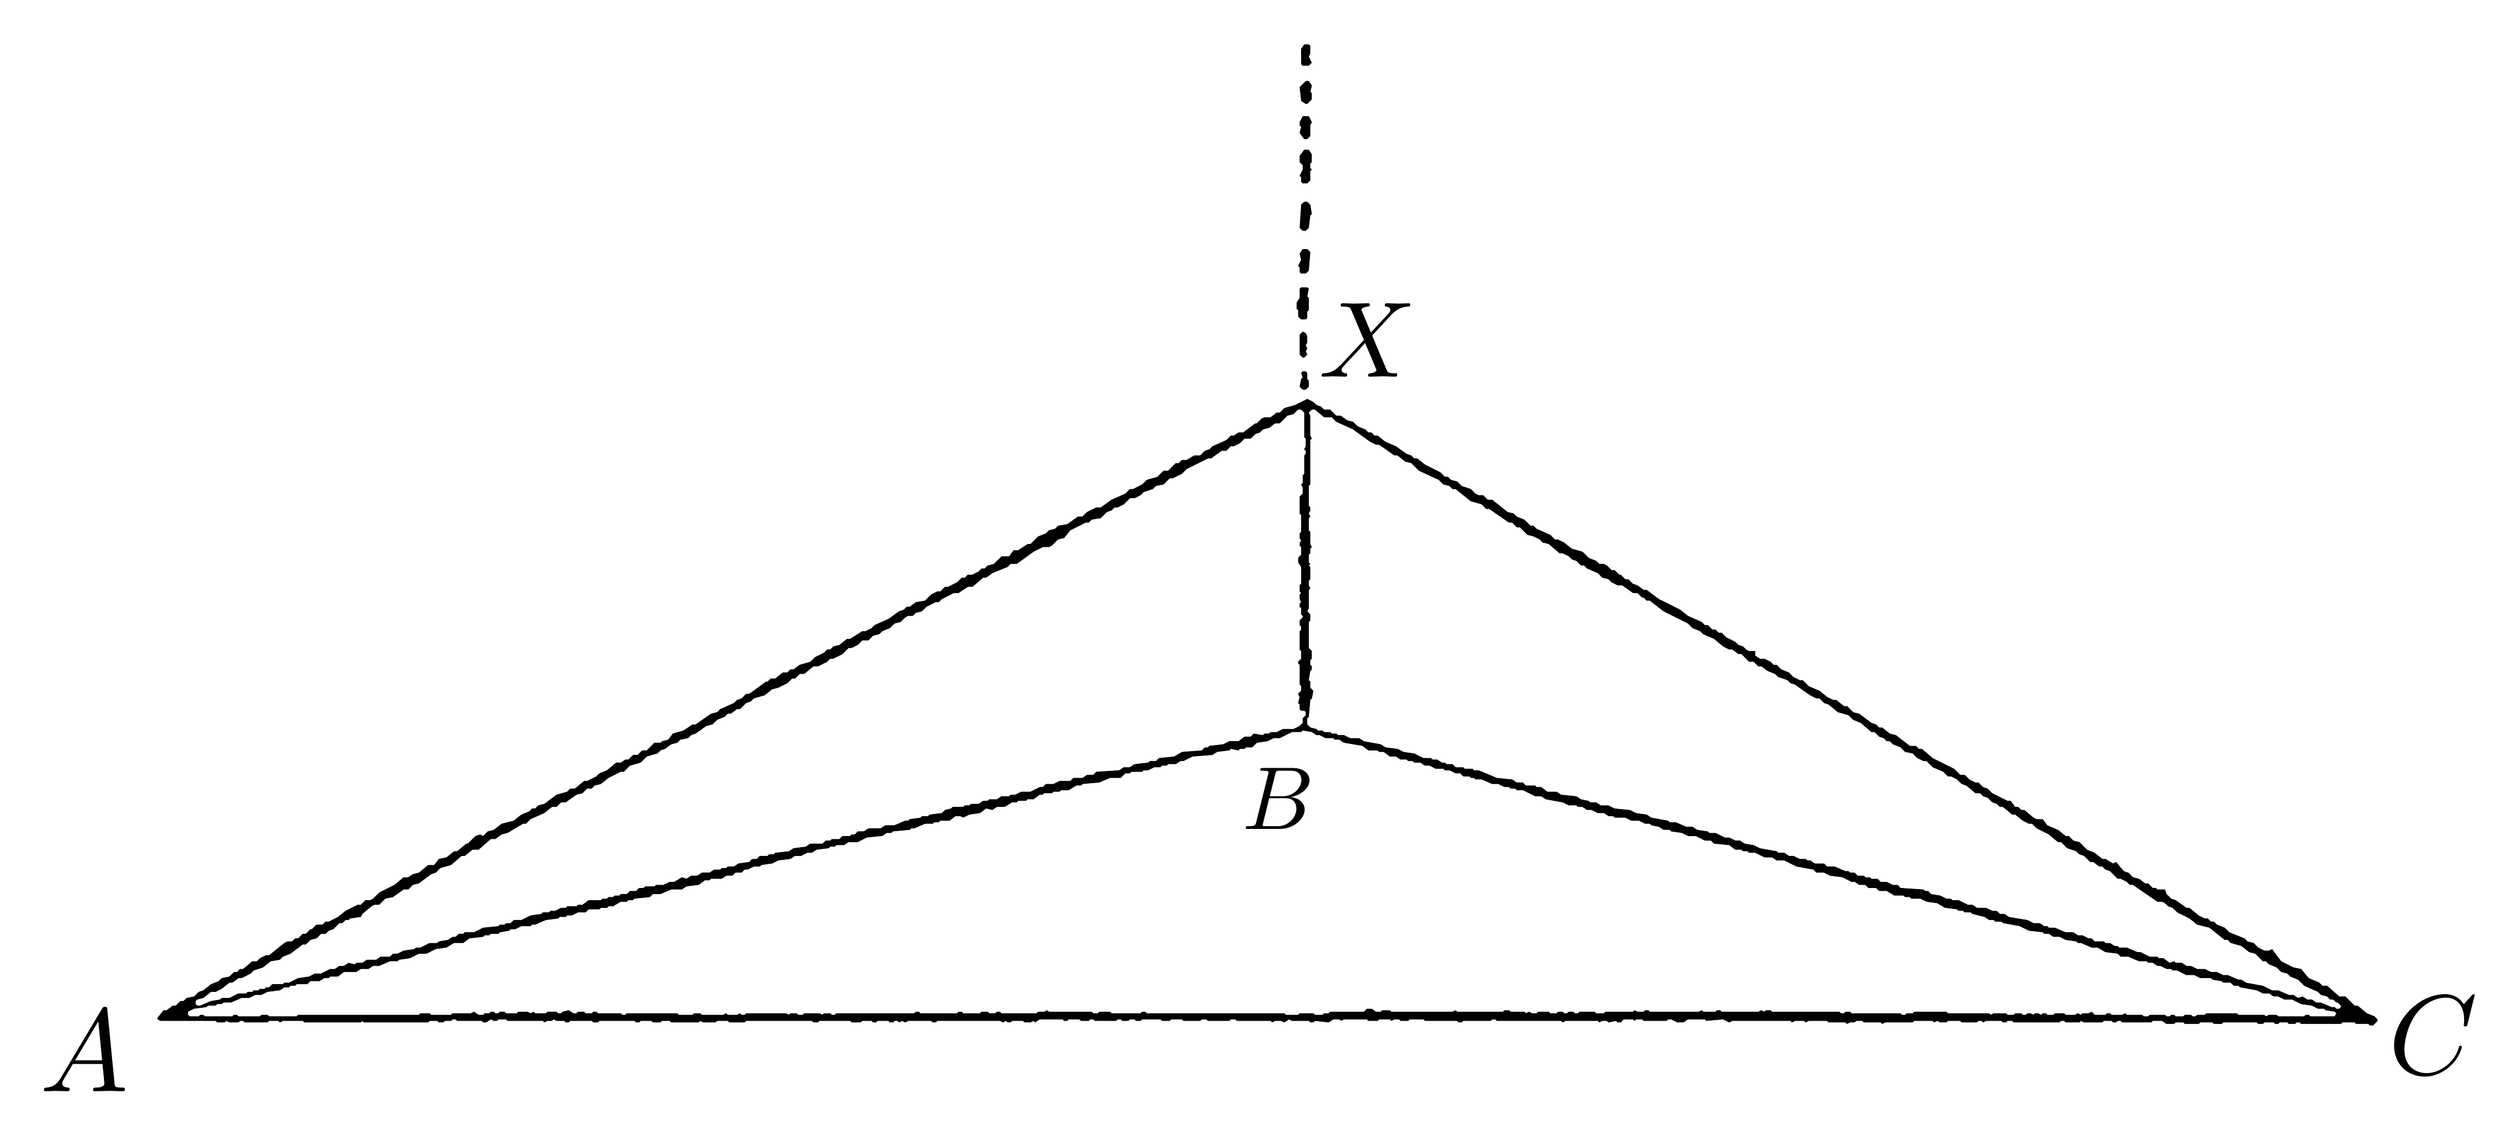
\begin{tikzpicture}[x=1pt,y=-1pt]
\path[use as bounding box] (0,0) rectangle (1615,720);
\path[fill=black,draw=none,even odd rule]
(1545,658) -- (1545,657) -- (1543,655) -- (1538,653) -- (1532,648) -- (1530,648) -- (1524,642) -- (1520,642) -- (1512,635) -- (1509,635) -- (1507,633) -- (1500,630) -- (1495,624) -- (1490,623) -- (1482,619) -- (1476,611) -- (1474,612) -- (1471,612) -- (1467,610) -- (1464,607) -- (1460,606) -- (1458,604) -- (1448,600) -- (1445,597) -- (1440,595) -- (1438,593) -- (1436,593) -- (1434,591) -- (1432,591) -- (1428,589) -- (1422,584) -- (1420,584) -- (1413,579) -- (1410,578) -- (1407,575) -- (1406,572) -- (1401,572) -- (1400,571) -- (1398,571) -- (1395,568) -- (1393,568) -- (1389,565) -- (1385,564) -- (1382,561) -- (1379,560) -- (1374,554) -- (1372,555) -- (1367,552) -- (1365,552) -- (1360,548) -- (1355,546) -- (1350,541) -- (1346,540) -- (1343,537) -- (1341,537) -- (1336,533) -- (1329,530) -- (1326,526) -- (1322,526) -- (1320,525) -- (1314,520) -- (1312,520) -- (1310,518) -- (1308,518) -- (1305,514) -- (1303,514) -- (1293,509) -- (1290,506) -- (1287,505) -- (1284,502) -- (1282,502) -- (1278,500) -- (1275,497) -- (1272,497) -- (1268,493) -- (1254,486) -- (1247,480) -- (1245,480) -- (1243,478) -- (1239,478) -- (1230,471) -- (1226,470) -- (1221,466) -- (1219,466) -- (1217,464) -- (1214,463) -- (1206,457) -- (1202,456) -- (1198,452) -- (1196,452) -- (1191,448) -- (1189,448) -- (1185,446) -- (1180,442) -- (1173,439) -- (1169,435) -- (1167,435) -- (1163,433) -- (1160,430) -- (1155,428) -- (1152,425) -- (1150,425) -- (1148,423) -- (1144,421) -- (1141,421) -- (1138,419) -- (1138,416) -- (1134,416) -- (1132,415) -- (1130,413) -- (1127,412) -- (1125,410) -- (1119,407) -- (1116,404) -- (1114,404) -- (1112,402) -- (1110,402) -- (1107,399) -- (1105,399) -- (1103,397) -- (1094,393) -- (1089,389) -- (1075,382) -- (1067,376) -- (1065,376) -- (1061,373) -- (1058,372) -- (1055,369) -- (1053,369) -- (1050,366) -- (1049,366) -- (1046,363) -- (1044,363) -- (1041,360) -- (1039,359) -- (1036,359) -- (1034,357) -- (1029,355) -- (1025,351) -- (1018,349) -- (1013,345) -- (1009,343) -- (1007,343) -- (1004,340) -- (995,336) -- (993,334) -- (991,334) -- (987,330) -- (982,328) -- (980,326) -- (976,325) -- (966,317) -- (963,317) -- (960,314) -- (957,314) -- (955,313) -- (952,310) -- (946,308) -- (943,305) -- (939,304) -- (937,302) -- (935,302) -- (932,299) -- (922,294) -- (917,290) -- (915,290) -- (913,288) -- (910,287) -- (903,282) -- (896,279) -- (891,275) -- (889,275) -- (887,273) -- (885,273) -- (883,271) -- (878,269) -- (875,266) -- (871,265) -- (867,262) -- (864,262) -- (860,258) -- (856,258) -- (854,256) -- (851,255) -- (849,253) -- (845,251) -- (837,255) -- (830,257) -- (827,260) -- (825,260) -- (821,263) -- (817,263) -- (815,264) -- (812,267) -- (811,267) -- (803,273) -- (800,273) -- (797,275) -- (795,275) -- (792,278) -- (783,282) -- (781,284) -- (778,285) -- (775,288) -- (771,288) -- (766,291) -- (763,291) -- (761,293) -- (759,293) -- (754,298) -- (751,298) -- (747,302) -- (740,304) -- (737,307) -- (731,310) -- (729,310) -- (726,313) -- (717,317) -- (710,322) -- (707,322) -- (701,325) -- (698,328) -- (695,328) -- (688,333) -- (682,334) -- (680,336) -- (676,337) -- (674,339) -- (669,341) -- (664,346) -- (662,346) -- (656,350) -- (653,350) -- (650,354) -- (645,354) -- (640,359) -- (636,360) -- (634,362) -- (632,362) -- (630,364) -- (626,366) -- (623,366) -- (621,368) -- (619,368) -- (616,371) -- (610,374) -- (608,374) -- (605,377) -- (603,377) -- (599,379) -- (595,383) -- (589,384) -- (585,387) -- (583,387) -- (581,389) -- (578,390) -- (571,395) -- (562,399) -- (560,401) -- (556,403) -- (554,403) -- (546,408) -- (544,408) -- (539,412) -- (535,413) -- (533,415) -- (531,415) -- (529,417) -- (523,420) -- (520,423) -- (513,425) -- (509,428) -- (507,428) -- (505,430) -- (502,430) -- (497,434) -- (494,434) -- (492,436) -- (491,436) -- (480,444) -- (478,444) -- (475,447) -- (472,448) -- (470,450) -- (461,454) -- (459,456) -- (455,457) -- (445,464) -- (443,464) -- (437,468) -- (430,470) -- (427,474) -- (423,475) -- (422,476) -- (418,476) -- (413,481) -- (410,481) -- (407,484) -- (404,484) -- (401,487) -- (399,487) -- (396,489) -- (393,489) -- (387,494) -- (382,496) -- (380,498) -- (374,501) -- (372,501) -- (366,506) -- (363,506) -- (361,508) -- (354,510) -- (346,516) -- (342,517) -- (340,519) -- (338,519) -- (336,521) -- (331,523) -- (326,527) -- (318,529) -- (313,533) -- (309,534) -- (306,537) -- (304,536) -- (301,537) -- (296,542) -- (295,542) -- (289,547) -- (287,547) -- (282,551) -- (277,552) -- (274,556) -- (270,556) -- (264,561) -- (260,562) -- (257,564) -- (254,564) -- (248,569) -- (238,574) -- (234,578) -- (232,579) -- (229,579) -- (226,582) -- (224,582) -- (216,586) -- (211,590) -- (205,593) -- (203,593) -- (201,595) -- (197,595) -- (194,598) -- (193,598) -- (190,601) -- (188,601) -- (185,604) -- (183,604) -- (181,606) -- (178,606) -- (176,607) -- (166,615) -- (164,615) -- (160,617) -- (158,619) -- (155,619) -- (149,624) -- (147,624) -- (145,626) -- (143,626) -- (140,629) -- (135,630) -- (133,632) -- (128,634) -- (123,638) -- (120,639) -- (117,642) -- (112,643) -- (110,645) -- (108,645) -- (105,648) -- (103,648) -- (99,651) -- (97,651) -- (93,656) -- (93,657) -- (95,658) -- (131,658) -- (132,659) -- (137,659) -- (138,658) -- (140,659) -- (146,659) -- (147,658) -- (149,658) -- (150,659) -- (165,659) -- (166,658) -- (172,658) -- (173,659) -- (175,658) -- (188,658) -- (189,659) -- (226,659) -- (227,658) -- (228,659) -- (270,659) -- (271,658) -- (276,658) -- (277,659) -- (280,659) -- (281,658) -- (285,658) -- (286,657) -- (288,657) -- (289,658) -- (305,658) -- (306,659) -- (308,659) -- (311,657) -- (313,658) -- (315,658) -- (316,657) -- (321,657) -- (322,658) -- (345,658) -- (346,659) -- (348,658) -- (351,658) -- (352,657) -- (354,658) -- (359,658) -- (360,659) -- (362,659) -- (363,658) -- (377,658) -- (378,659) -- (381,659) -- (382,658) -- (405,658) -- (406,659) -- (408,659) -- (409,658) -- (416,658) -- (417,659) -- (422,659) -- (423,658) -- (428,658) -- (429,659) -- (447,659) -- (448,658) -- (450,659) -- (458,659) -- (459,658) -- (466,658) -- (467,659) -- (477,659) -- (478,658) -- (521,658) -- (522,659) -- (525,659) -- (526,658) -- (546,658) -- (547,659) -- (553,659) -- (554,658) -- (560,658) -- (561,659) -- (563,659) -- (564,658) -- (571,658) -- (572,659) -- (574,659) -- (575,658) -- (577,658) -- (578,659) -- (580,658) -- (582,659) -- (584,658) -- (599,658) -- (600,659) -- (602,659) -- (603,658) -- (644,658) -- (646,659) -- (648,658) -- (649,659) -- (651,659) -- (652,658) -- (659,658) -- (660,659) -- (664,659) -- (666,658) -- (667,659) -- (670,657) -- (685,657) -- (686,658) -- (688,658) -- (689,657) -- (696,657) -- (697,658) -- (702,658) -- (703,657) -- (705,657) -- (706,658) -- (720,658) -- (721,657) -- (723,657) -- (724,658) -- (728,658) -- (729,657) -- (732,657) -- (733,658) -- (736,658) -- (737,657) -- (749,657) -- (750,658) -- (755,658) -- (756,657) -- (763,657) -- (764,658) -- (775,658) -- (776,657) -- (779,657) -- (780,658) -- (794,658) -- (795,657) -- (798,657) -- (799,658) -- (821,658) -- (822,659) -- (824,658) -- (828,658) -- (830,659) -- (833,657) -- (835,658) -- (846,658) -- (847,659) -- (849,659) -- (850,658) -- (859,659) -- (862,657) -- (866,657) -- (867,658) -- (869,657) -- (884,657) -- (885,658) -- (891,658) -- (892,657) -- (899,657) -- (900,658) -- (902,657) -- (905,657) -- (906,658) -- (911,658) -- (912,657) -- (921,657) -- (922,658) -- (943,658) -- (944,659) -- (946,659) -- (947,658) -- (965,658) -- (966,657) -- (968,657) -- (969,658) -- (1011,658) -- (1012,659) -- (1014,658) -- (1035,658) -- (1036,659) -- (1038,658) -- (1041,658) -- (1042,659) -- (1047,658) -- (1048,659) -- (1050,659) -- (1052,657) -- (1058,657) -- (1059,658) -- (1060,657) -- (1064,657) -- (1065,658) -- (1080,658) -- (1081,657) -- (1083,657) -- (1087,659) -- (1091,659) -- (1094,657) -- (1105,657) -- (1106,658) -- (1117,657) -- (1121,659) -- (1123,658) -- (1161,658) -- (1162,659) -- (1164,658) -- (1170,658) -- (1171,659) -- (1173,658) -- (1185,658) -- (1186,659) -- (1197,659) -- (1198,660) -- (1200,659) -- (1203,659) -- (1204,658) -- (1208,658) -- (1209,659) -- (1220,659) -- (1221,660) -- (1223,659) -- (1241,659) -- (1242,658) -- (1254,658) -- (1255,659) -- (1257,658) -- (1259,659) -- (1263,659) -- (1264,658) -- (1272,658) -- (1273,659) -- (1283,659) -- (1284,658) -- (1286,658) -- (1287,659) -- (1289,658) -- (1299,658) -- (1300,659) -- (1302,659) -- (1303,658) -- (1306,658) -- (1307,659) -- (1337,659) -- (1338,658) -- (1340,658) -- (1341,659) -- (1350,659) -- (1351,658) -- (1353,659) -- (1365,659) -- (1366,658) -- (1371,658) -- (1372,659) -- (1374,659) -- (1375,658) -- (1377,658) -- (1378,659) -- (1397,659) -- (1398,658) -- (1404,658) -- (1407,660) -- (1412,660) -- (1413,659) -- (1418,659) -- (1419,660) -- (1428,660) -- (1429,659) -- (1437,659) -- (1438,660) -- (1443,660) -- (1444,659) -- (1466,659) -- (1467,660) -- (1470,660) -- (1471,659) -- (1477,659) -- (1478,660) -- (1480,660) -- (1481,659) -- (1486,659) -- (1487,660) -- (1491,660) -- (1492,659) -- (1494,659) -- (1495,660) -- (1521,660) -- (1522,659) -- (1530,659) -- (1531,660) -- (1539,660) -- (1540,661) -- (1542,661) -- cycle
(1518,653) -- (1517,655) -- (1501,655) -- (1500,654) -- (1498,654) -- (1497,655) -- (1480,655) -- (1479,654) -- (1474,654) -- (1472,655) -- (1471,654) -- (1454,654) -- (1453,653) -- (1433,653) -- (1432,654) -- (1427,654) -- (1426,655) -- (1424,655) -- (1423,654) -- (1419,654) -- (1418,655) -- (1413,655) -- (1412,654) -- (1410,654) -- (1409,655) -- (1407,655) -- (1406,654) -- (1396,654) -- (1395,655) -- (1392,655) -- (1391,654) -- (1381,654) -- (1380,653) -- (1378,654) -- (1371,654) -- (1370,653) -- (1368,653) -- (1367,654) -- (1360,654) -- (1358,652) -- (1356,653) -- (1352,653) -- (1351,654) -- (1349,653) -- (1347,654) -- (1341,654) -- (1340,653) -- (1334,653) -- (1333,654) -- (1329,654) -- (1328,653) -- (1326,653) -- (1325,654) -- (1323,653) -- (1321,653) -- (1320,654) -- (1318,653) -- (1316,653) -- (1315,654) -- (1313,654) -- (1312,653) -- (1308,653) -- (1307,654) -- (1303,654) -- (1302,653) -- (1294,653) -- (1292,654) -- (1291,653) -- (1264,653) -- (1263,652) -- (1242,652) -- (1241,653) -- (1237,653) -- (1236,654) -- (1234,654) -- (1233,653) -- (1201,653) -- (1200,652) -- (1197,652) -- (1196,653) -- (1194,653) -- (1193,652) -- (1149,652) -- (1148,651) -- (1145,651) -- (1144,652) -- (1142,651) -- (1140,652) -- (1116,652) -- (1115,651) -- (1113,651) -- (1112,652) -- (1104,652) -- (1103,651) -- (1101,652) -- (1069,652) -- (1068,651) -- (1066,651) -- (1065,652) -- (1061,652) -- (1059,651) -- (1058,652) -- (1040,652) -- (1039,653) -- (1034,653) -- (1033,652) -- (1023,652) -- (1022,653) -- (1020,653) -- (1019,652) -- (1016,652) -- (1015,653) -- (1013,653) -- (1012,652) -- (1009,652) -- (1008,653) -- (1004,653) -- (1003,652) -- (996,652) -- (995,653) -- (992,653) -- (990,652) -- (988,653) -- (987,652) -- (978,652) -- (977,651) -- (974,651) -- (973,652) -- (943,652) -- (942,651) -- (940,652) -- (900,652) -- (899,651) -- (894,651) -- (893,652) -- (890,652) -- (887,650) -- (884,650) -- (882,652) -- (860,652) -- (859,653) -- (856,653) -- (855,654) -- (850,654) -- (849,653) -- (840,653) -- (839,654) -- (831,654) -- (830,653) -- (740,653) -- (739,652) -- (737,652) -- (736,653) -- (717,653) -- (716,652) -- (709,652) -- (708,653) -- (705,653) -- (704,652) -- (676,652) -- (675,651) -- (673,652) -- (669,652) -- (668,653) -- (645,653) -- (644,652) -- (642,652) -- (641,653) -- (637,653) -- (636,652) -- (632,652) -- (631,653) -- (620,653) -- (619,652) -- (617,652) -- (616,653) -- (592,653) -- (591,652) -- (589,652) -- (588,653) -- (537,653) -- (536,654) -- (534,654) -- (533,653) -- (529,653) -- (528,654) -- (526,653) -- (516,653) -- (515,654) -- (512,654) -- (511,653) -- (507,653) -- (506,654) -- (504,653) -- (478,653) -- (477,654) -- (475,654) -- (474,653) -- (472,654) -- (466,654) -- (465,653) -- (463,654) -- (449,654) -- (448,653) -- (444,653) -- (443,654) -- (434,654) -- (433,653) -- (400,653) -- (399,654) -- (397,654) -- (396,653) -- (381,653) -- (380,652) -- (378,652) -- (377,653) -- (373,653) -- (372,652) -- (368,652) -- (367,653) -- (365,653) -- (362,651) -- (358,652) -- (357,653) -- (355,653) -- (354,652) -- (348,652) -- (347,653) -- (340,653) -- (339,652) -- (337,653) -- (335,652) -- (329,652) -- (328,653) -- (321,653) -- (320,652) -- (317,652) -- (316,653) -- (314,653) -- (313,652) -- (311,652) -- (310,653) -- (307,653) -- (306,654) -- (303,654) -- (300,652) -- (298,653) -- (286,653) -- (285,654) -- (272,654) -- (271,653) -- (265,653) -- (264,654) -- (185,654) -- (184,655) -- (166,655) -- (165,654) -- (161,654) -- (160,655) -- (146,655) -- (145,654) -- (143,654) -- (142,655) -- (124,655) -- (123,654) -- (121,654) -- (120,655) -- (114,655) -- (113,654) -- (113,652) -- (117,650) -- (125,649) -- (126,648) -- (131,648) -- (132,647) -- (135,647) -- (136,646) -- (141,646) -- (148,643) -- (153,643) -- (157,641) -- (161,641) -- (165,639) -- (173,638) -- (176,636) -- (179,636) -- (180,635) -- (183,635) -- (184,634) -- (191,634) -- (193,632) -- (199,632) -- (202,630) -- (205,630) -- (206,629) -- (211,629) -- (215,626) -- (223,626) -- (226,624) -- (231,624) -- (234,622) -- (238,622) -- (245,619) -- (250,619) -- (251,618) -- (258,617) -- (264,614) -- (269,614) -- (275,611) -- (282,610) -- (287,607) -- (293,607) -- (297,604) -- (306,603) -- (307,602) -- (310,602) -- (311,601) -- (316,601) -- (317,600) -- (323,599) -- (324,598) -- (327,598) -- (331,596) -- (337,596) -- (338,595) -- (340,595) -- (347,592) -- (355,591) -- (356,590) -- (360,590) -- (361,589) -- (364,589) -- (368,587) -- (373,587) -- (375,585) -- (382,585) -- (383,584) -- (387,584) -- (388,583) -- (391,583) -- (396,580) -- (400,580) -- (401,579) -- (404,579) -- (405,578) -- (415,577) -- (417,575) -- (422,575) -- (429,572) -- (436,572) -- (439,570) -- (447,569) -- (451,566) -- (454,566) -- (455,565) -- (462,565) -- (465,563) -- (469,563) -- (471,561) -- (475,561) -- (477,559) -- (479,559) -- (483,557) -- (487,557) -- (488,556) -- (495,555) -- (499,553) -- (507,552) -- (510,550) -- (514,550) -- (518,548) -- (521,548) -- (524,546) -- (532,545) -- (533,544) -- (536,544) -- (537,543) -- (542,543) -- (545,541) -- (551,541) -- (557,538) -- (567,537) -- (570,535) -- (573,535) -- (574,534) -- (585,533) -- (586,532) -- (588,532) -- (595,529) -- (600,529) -- (601,528) -- (604,528) -- (605,527) -- (611,527) -- (615,524) -- (618,524) -- (620,525) -- (624,523) -- (631,522) -- (635,519) -- (639,520) -- (642,518) -- (647,518) -- (652,515) -- (655,515) -- (656,514) -- (661,514) -- (662,513) -- (666,513) -- (670,510) -- (672,510) -- (673,509) -- (678,509) -- (679,508) -- (683,508) -- (684,507) -- (689,507) -- (694,504) -- (697,504) -- (698,503) -- (709,502) -- (716,499) -- (723,499) -- (726,496) -- (729,496) -- (730,495) -- (737,495) -- (738,494) -- (741,494) -- (745,492) -- (749,492) -- (750,491) -- (753,491) -- (754,490) -- (759,490) -- (762,488) -- (764,488) -- (770,485) -- (783,484) -- (786,482) -- (794,481) -- (795,480) -- (800,481) -- (801,480) -- (804,480) -- (805,479) -- (809,479) -- (812,476) -- (819,475) -- (823,473) -- (827,473) -- (835,469) -- (841,469) -- (842,468) -- (848,469) -- (851,471) -- (853,471) -- (857,473) -- (862,473) -- (863,474) -- (866,474) -- (869,476) -- (881,478) -- (885,481) -- (891,481) -- (892,482) -- (895,482) -- (899,485) -- (903,485) -- (906,487) -- (910,487) -- (911,488) -- (914,488) -- (915,489) -- (919,489) -- (922,491) -- (925,491) -- (929,493) -- (934,493) -- (935,494) -- (938,494) -- (942,496) -- (945,496) -- (947,498) -- (951,498) -- (952,499) -- (954,499) -- (955,500) -- (959,500) -- (966,503) -- (970,503) -- (974,505) -- (977,505) -- (978,506) -- (981,506) -- (982,507) -- (986,507) -- (994,511) -- (998,511) -- (1001,513) -- (1012,515) -- (1016,517) -- (1021,517) -- (1022,518) -- (1025,518) -- (1028,520) -- (1031,520) -- (1035,522) -- (1039,522) -- (1042,524) -- (1045,524) -- (1046,525) -- (1053,525) -- (1057,527) -- (1062,527) -- (1066,529) -- (1069,529) -- (1070,530) -- (1075,531) -- (1078,533) -- (1082,533) -- (1083,534) -- (1090,535) -- (1094,537) -- (1099,537) -- (1105,540) -- (1109,540) -- (1111,542) -- (1121,543) -- (1125,546) -- (1129,546) -- (1130,547) -- (1133,547) -- (1134,548) -- (1138,548) -- (1144,551) -- (1149,551) -- (1152,553) -- (1157,553) -- (1165,557) -- (1176,559) -- (1178,561) -- (1183,561) -- (1187,563) -- (1195,564) -- (1201,567) -- (1203,567) -- (1206,569) -- (1210,569) -- (1212,571) -- (1217,571) -- (1219,573) -- (1224,573) -- (1229,576) -- (1235,576) -- (1236,577) -- (1239,577) -- (1240,578) -- (1246,578) -- (1250,580) -- (1257,581) -- (1262,584) -- (1270,585) -- (1271,586) -- (1274,586) -- (1275,587) -- (1279,587) -- (1280,588) -- (1288,590) -- (1291,592) -- (1294,592) -- (1295,593) -- (1299,593) -- (1300,594) -- (1311,596) -- (1317,599) -- (1326,600) -- (1327,601) -- (1330,601) -- (1333,603) -- (1337,603) -- (1341,605) -- (1348,606) -- (1349,607) -- (1351,607) -- (1358,610) -- (1362,610) -- (1367,613) -- (1375,614) -- (1377,616) -- (1382,616) -- (1389,619) -- (1394,619) -- (1395,620) -- (1398,620) -- (1401,622) -- (1403,622) -- (1407,624) -- (1410,624) -- (1411,625) -- (1414,625) -- (1420,628) -- (1425,628) -- (1429,630) -- (1436,630) -- (1437,631) -- (1443,632) -- (1444,633) -- (1449,633) -- (1451,635) -- (1454,635) -- (1455,636) -- (1466,638) -- (1470,640) -- (1474,640) -- (1477,642) -- (1480,642) -- (1484,644) -- (1489,644) -- (1495,647) -- (1502,648) -- (1506,650) -- (1510,650) -- (1511,651) -- (1517,652) -- cycle
(846,260) -- (848,258) -- (850,258) -- (856,263) -- (861,263) -- (864,266) -- (875,271) -- (886,279) -- (890,281) -- (892,281) -- (902,288) -- (904,288) -- (909,292) -- (913,293) -- (918,298) -- (931,304) -- (934,307) -- (938,308) -- (940,310) -- (942,310) -- (952,318) -- (959,320) -- (962,323) -- (964,323) -- (977,332) -- (979,332) -- (982,335) -- (984,335) -- (989,340) -- (993,341) -- (997,343) -- (999,345) -- (1003,346) -- (1010,352) -- (1012,352) -- (1016,354) -- (1018,356) -- (1021,357) -- (1024,360) -- (1026,360) -- (1028,362) -- (1035,365) -- (1038,368) -- (1042,369) -- (1044,371) -- (1048,373) -- (1051,373) -- (1058,378) -- (1061,378) -- (1064,381) -- (1065,381) -- (1067,383) -- (1069,383) -- (1078,390) -- (1094,398) -- (1097,401) -- (1102,403) -- (1104,405) -- (1111,408) -- (1117,413) -- (1121,415) -- (1123,415) -- (1127,418) -- (1129,418) -- (1134,423) -- (1137,423) -- (1140,426) -- (1142,426) -- (1146,429) -- (1151,431) -- (1153,433) -- (1159,435) -- (1161,437) -- (1164,438) -- (1174,445) -- (1178,447) -- (1180,447) -- (1183,450) -- (1186,451) -- (1192,456) -- (1199,458) -- (1202,461) -- (1207,463) -- (1214,469) -- (1216,469) -- (1219,472) -- (1222,473) -- (1224,475) -- (1226,475) -- (1228,477) -- (1233,479) -- (1236,482) -- (1241,483) -- (1244,486) -- (1248,488) -- (1250,488) -- (1254,492) -- (1261,495) -- (1264,498) -- (1266,498) -- (1270,500) -- (1273,503) -- (1276,504) -- (1282,509) -- (1285,509) -- (1287,511) -- (1290,512) -- (1293,515) -- (1296,516) -- (1298,518) -- (1300,518) -- (1306,523) -- (1308,523) -- (1313,527) -- (1317,529) -- (1319,529) -- (1322,532) -- (1330,536) -- (1336,541) -- (1338,541) -- (1342,545) -- (1348,547) -- (1350,549) -- (1353,550) -- (1357,554) -- (1359,554) -- (1363,557) -- (1365,557) -- (1367,559) -- (1370,560) -- (1375,565) -- (1377,565) -- (1381,567) -- (1383,569) -- (1385,569) -- (1401,580) -- (1404,580) -- (1406,581) -- (1408,583) -- (1411,584) -- (1414,587) -- (1422,591) -- (1427,595) -- (1435,597) -- (1445,605) -- (1447,605) -- (1449,607) -- (1456,609) -- (1461,613) -- (1465,614) -- (1470,619) -- (1472,619) -- (1474,621) -- (1479,623) -- (1482,626) -- (1486,627) -- (1488,629) -- (1493,631) -- (1497,635) -- (1506,639) -- (1508,641) -- (1512,642) -- (1514,644) -- (1516,644) -- (1518,646) -- (1519,646) -- (1521,648) -- (1521,649) -- (1520,650) -- (1518,650) -- (1517,649) -- (1515,649) -- (1508,646) -- (1505,646) -- (1502,644) -- (1499,644) -- (1496,642) -- (1493,643) -- (1490,641) -- (1487,641) -- (1480,638) -- (1476,638) -- (1470,635) -- (1459,633) -- (1456,631) -- (1454,631) -- (1447,628) -- (1444,628) -- (1440,626) -- (1436,626) -- (1432,624) -- (1427,624) -- (1423,622) -- (1420,622) -- (1417,620) -- (1413,620) -- (1412,619) -- (1409,620) -- (1405,617) -- (1402,617) -- (1401,616) -- (1396,616) -- (1390,613) -- (1388,613) -- (1381,610) -- (1376,610) -- (1375,609) -- (1373,609) -- (1370,607) -- (1367,607) -- (1366,606) -- (1360,606) -- (1358,604) -- (1356,604) -- (1352,602) -- (1349,602) -- (1346,600) -- (1341,600) -- (1334,597) -- (1330,597) -- (1329,596) -- (1327,596) -- (1324,594) -- (1320,594) -- (1316,592) -- (1304,590) -- (1301,588) -- (1298,588) -- (1296,586) -- (1293,586) -- (1289,584) -- (1283,584) -- (1280,582) -- (1277,582) -- (1271,579) -- (1267,579) -- (1266,578) -- (1263,578) -- (1259,576) -- (1253,575) -- (1251,573) -- (1249,573) -- (1248,572) -- (1233,571) -- (1231,569) -- (1228,569) -- (1224,567) -- (1220,567) -- (1218,565) -- (1214,565) -- (1213,564) -- (1210,564) -- (1209,563) -- (1205,563) -- (1203,561) -- (1200,561) -- (1199,560) -- (1197,560) -- (1190,557) -- (1185,557) -- (1183,555) -- (1177,555) -- (1174,553) -- (1172,553) -- (1171,552) -- (1167,552) -- (1163,550) -- (1160,550) -- (1157,548) -- (1153,548) -- (1152,547) -- (1141,545) -- (1137,543) -- (1131,542) -- (1128,540) -- (1125,540) -- (1121,538) -- (1118,538) -- (1112,535) -- (1108,535) -- (1107,534) -- (1100,533) -- (1097,531) -- (1093,531) -- (1086,528) -- (1082,528) -- (1081,527) -- (1070,525) -- (1067,523) -- (1060,522) -- (1056,520) -- (1046,519) -- (1042,517) -- (1037,517) -- (1034,515) -- (1030,515) -- (1029,514) -- (1024,513) -- (1021,511) -- (1011,510) -- (1008,508) -- (1002,508) -- (998,505) -- (995,505) -- (994,504) -- (988,504) -- (986,502) -- (982,502) -- (979,500) -- (969,499) -- (957,494) -- (954,494) -- (953,493) -- (948,493) -- (947,492) -- (942,492) -- (940,490) -- (936,490) -- (935,489) -- (933,489) -- (930,487) -- (927,487) -- (926,486) -- (921,486) -- (915,483) -- (908,482) -- (904,480) -- (896,479) -- (893,477) -- (882,475) -- (879,473) -- (873,473) -- (869,471) -- (865,471) -- (864,470) -- (861,470) -- (860,469) -- (856,469) -- (855,468) -- (852,468) -- (851,467) -- (847,466) -- (845,464) -- (845,460) -- (846,459) -- (847,448) -- (848,447) -- (849,442) -- (847,440) -- (847,436) -- (846,435) -- (847,429) -- (848,428) -- (848,426) -- (847,425) -- (847,422) -- (848,421) -- (848,416) -- (846,414) -- (846,397) -- (847,396) -- (847,392) -- (845,390) -- (846,388) -- (846,376) -- (847,375) -- (846,373) -- (846,370) -- (847,369) -- (847,361) -- (846,360) -- (847,359) -- (846,358) -- (846,353) -- (847,352) -- (847,349) -- (848,348) -- (847,346) -- (847,338) -- (846,337) -- (846,329) -- (847,328) -- (846,326) -- (847,324) -- (847,322) -- (846,321) -- (846,308) -- (847,307) -- (847,278) -- (848,277) -- (847,275) -- (847,262) -- cycle
(843,260) -- (843,276) -- (844,277) -- (844,282) -- (843,284) -- (844,285) -- (844,287) -- (843,288) -- (843,300) -- (842,301) -- (842,306) -- (841,307) -- (842,309) -- (842,313) -- (840,315) -- (840,326) -- (841,327) -- (841,338) -- (840,339) -- (840,342) -- (841,344) -- (840,345) -- (840,347) -- (841,348) -- (841,353) -- (839,355) -- (839,358) -- (841,361) -- (841,372) -- (840,373) -- (840,377) -- (841,378) -- (840,379) -- (840,382) -- (841,384) -- (840,385) -- (840,387) -- (841,388) -- (841,392) -- (842,393) -- (842,394) -- (840,396) -- (840,399) -- (841,400) -- (841,402) -- (840,403) -- (840,415) -- (841,416) -- (841,421) -- (839,423) -- (839,424) -- (840,425) -- (840,438) -- (841,439) -- (841,442) -- (839,444) -- (840,446) -- (839,450) -- (840,451) -- (840,454) -- (841,455) -- (843,455) -- (844,456) -- (844,458) -- (842,460) -- (842,463) -- (840,465) -- (836,467) -- (829,467) -- (825,469) -- (821,469) -- (820,470) -- (817,470) -- (816,471) -- (810,470) -- (808,472) -- (804,472) -- (800,475) -- (794,475) -- (790,477) -- (781,478) -- (780,479) -- (778,479) -- (776,481) -- (763,482) -- (758,485) -- (748,486) -- (746,488) -- (742,488) -- (741,489) -- (732,490) -- (729,492) -- (725,492) -- (722,494) -- (707,495) -- (705,497) -- (701,497) -- (698,499) -- (692,499) -- (690,501) -- (683,501) -- (679,503) -- (674,503) -- (672,505) -- (670,505) -- (664,508) -- (658,508) -- (654,510) -- (651,510) -- (650,511) -- (645,511) -- (642,513) -- (637,513) -- (636,514) -- (633,514) -- (630,516) -- (625,516) -- (624,517) -- (621,517) -- (620,518) -- (613,518) -- (612,519) -- (608,520) -- (606,522) -- (598,523) -- (597,524) -- (593,524) -- (592,525) -- (585,526) -- (584,527) -- (582,527) -- (575,530) -- (569,530) -- (566,532) -- (558,532) -- (555,534) -- (551,534) -- (549,536) -- (547,536) -- (546,537) -- (541,537) -- (539,539) -- (534,539) -- (533,540) -- (530,540) -- (528,542) -- (520,542) -- (517,544) -- (509,545) -- (506,547) -- (497,548) -- (496,549) -- (493,549) -- (492,550) -- (487,550) -- (485,552) -- (482,552) -- (480,554) -- (473,555) -- (470,557) -- (466,557) -- (465,558) -- (462,558) -- (461,559) -- (457,559) -- (454,561) -- (449,561) -- (446,563) -- (442,563) -- (439,565) -- (436,564) -- (431,567) -- (428,567) -- (424,569) -- (419,569) -- (418,570) -- (412,570) -- (411,571) -- (408,571) -- (406,573) -- (402,573) -- (400,575) -- (396,575) -- (395,576) -- (392,576) -- (391,577) -- (388,577) -- (387,578) -- (384,578) -- (383,579) -- (375,579) -- (371,582) -- (368,582) -- (367,583) -- (361,583) -- (360,584) -- (357,584) -- (353,586) -- (350,586) -- (349,587) -- (345,587) -- (344,588) -- (337,589) -- (331,592) -- (326,592) -- (324,594) -- (321,594) -- (320,595) -- (317,595) -- (316,596) -- (306,597) -- (300,600) -- (294,600) -- (293,601) -- (290,601) -- (288,603) -- (286,603) -- (283,605) -- (277,606) -- (276,607) -- (271,607) -- (265,610) -- (262,610) -- (261,611) -- (254,612) -- (250,614) -- (247,614) -- (245,616) -- (239,616) -- (236,618) -- (230,618) -- (227,620) -- (223,620) -- (222,621) -- (218,620) -- (215,622) -- (212,622) -- (209,624) -- (206,624) -- (200,627) -- (196,627) -- (192,629) -- (185,630) -- (179,633) -- (176,633) -- (175,634) -- (168,634) -- (166,636) -- (164,636) -- (163,637) -- (160,637) -- (159,638) -- (156,638) -- (155,639) -- (152,639) -- (151,640) -- (146,640) -- (140,643) -- (135,643) -- (134,644) -- (128,645) -- (121,648) -- (119,648) -- (118,647) -- (118,645) -- (119,644) -- (123,643) -- (128,639) -- (131,639) -- (135,637) -- (140,633) -- (142,633) -- (146,630) -- (148,630) -- (154,627) -- (156,625) -- (162,623) -- (167,619) -- (173,618) -- (175,616) -- (180,614) -- (188,608) -- (190,608) -- (193,605) -- (197,604) -- (200,601) -- (203,601) -- (205,599) -- (208,598) -- (212,594) -- (214,594) -- (216,592) -- (218,592) -- (219,591) -- (226,590) -- (227,588) -- (233,583) -- (235,582) -- (238,582) -- (242,578) -- (247,577) -- (254,572) -- (257,572) -- (260,569) -- (264,568) -- (272,562) -- (275,561) -- (278,558) -- (285,556) -- (292,550) -- (294,550) -- (299,546) -- (303,546) -- (311,539) -- (314,539) -- (318,536) -- (322,535) -- (332,529) -- (334,529) -- (337,526) -- (346,522) -- (351,518) -- (354,518) -- (357,515) -- (360,515) -- (367,510) -- (371,509) -- (374,506) -- (377,506) -- (379,504) -- (383,503) -- (388,499) -- (396,495) -- (398,495) -- (402,491) -- (409,489) -- (413,485) -- (420,483) -- (422,481) -- (425,480) -- (429,477) -- (433,476) -- (435,474) -- (440,473) -- (442,471) -- (445,470) -- (452,465) -- (456,464) -- (459,461) -- (464,459) -- (466,457) -- (468,457) -- (472,454) -- (474,454) -- (478,450) -- (481,449) -- (483,447) -- (490,445) -- (495,441) -- (499,440) -- (505,437) -- (508,434) -- (510,434) -- (513,431) -- (516,431) -- (522,426) -- (525,426) -- (531,423) -- (533,421) -- (535,421) -- (541,418) -- (545,414) -- (547,414) -- (551,412) -- (554,409) -- (558,409) -- (561,406) -- (565,405) -- (567,403) -- (572,401) -- (575,398) -- (579,397) -- (582,394) -- (584,393) -- (587,393) -- (589,391) -- (593,390) -- (596,387) -- (602,384) -- (604,384) -- (606,382) -- (614,378) -- (617,378) -- (623,374) -- (626,374) -- (633,368) -- (635,368) -- (639,365) -- (649,361) -- (651,359) -- (655,359) -- (666,351) -- (672,348) -- (676,348) -- (678,347) -- (682,343) -- (686,342) -- (690,337) -- (700,332) -- (702,332) -- (704,330) -- (710,329) -- (714,325) -- (717,324) -- (719,322) -- (721,322) -- (725,320) -- (729,316) -- (732,316) -- (736,314) -- (738,312) -- (744,310) -- (746,308) -- (751,307) -- (755,303) -- (757,303) -- (763,300) -- (766,297) -- (780,290) -- (782,290) -- (789,285) -- (792,285) -- (795,282) -- (797,282) -- (801,280) -- (804,277) -- (808,277) -- (811,274) -- (814,273) -- (816,271) -- (820,270) -- (824,267) -- (827,267) -- (832,262) -- (836,261) -- (839,258) -- (841,258) -- cycle
(842,233) -- (841,234) -- (842,237) -- (841,238) -- (840,243) -- (842,245) -- (844,245) -- (846,243) -- (846,239) -- (845,238) -- (845,234) -- (844,233) -- cycle
(842,207) -- (840,209) -- (840,222) -- (842,224) -- (843,224) -- (845,222) -- (844,220) -- (845,218) -- (844,216) -- (845,214) -- (845,210) -- (844,208) -- cycle
(841,178) -- (840,179) -- (840,185) -- (838,188) -- (838,192) -- (839,193) -- (839,197) -- (841,199) -- (844,199) -- (845,198) -- (845,194) -- (846,193) -- (846,185) -- (845,184) -- (846,179) -- (845,178) -- cycle
(842,153) -- (840,156) -- (841,160) -- (839,164) -- (840,165) -- (840,168) -- (841,169) -- (844,169) -- (846,167) -- (847,155) -- (845,153) -- cycle
(845,122) -- (843,122) -- (841,124) -- (840,139) -- (842,141) -- (844,141) -- (846,139) -- (847,131) -- (848,130) -- (847,124) -- cycle
(843,88) -- (840,92) -- (840,96) -- (842,98) -- (842,101) -- (840,105) -- (841,106) -- (841,109) -- (842,110) -- (845,110) -- (847,108) -- (847,102) -- (848,101) -- (847,100) -- (847,97) -- (848,96) -- (848,91) -- (846,88) -- cycle
(842,66) -- (840,70) -- (840,72) -- (841,73) -- (840,77) -- (843,81) -- (845,81) -- (847,79) -- (847,72) -- (848,70) -- (846,66) -- cycle
(846,43) -- (844,43) -- (840,47) -- (841,56) -- (844,58) -- (845,58) -- (848,55) -- (848,51) -- (847,50) -- (848,46) -- cycle
(843,19) -- (841,22) -- (841,32) -- (842,33) -- (846,33) -- (848,31) -- (846,27) -- (847,25) -- (847,20) -- (846,19) -- cycle;
\node[inner sep=0pt,font=\fontsize{10}{10}\selectfont] at (884.5,212.5) {\scalebox{7.029}{$X$}};
\node[inner sep=0pt,font=\fontsize{10}{10}\selectfont] at (826.0,512.5) {\scalebox{5.841}{$B$}};
\node[inner sep=0pt,font=\fontsize{10}{10}\selectfont] at (45.0,678.0) {\scalebox{7.722}{$A$}};
\node[inner sep=0pt,font=\fontsize{10}{10}\selectfont] at (1581.5,667.5) {\scalebox{7.425}{$C$}};
\end{tikzpicture}%
}
\end{center}

Hier würde Ihnen die Rechnung den Punkt $X$ geben, der aber nur
passt, wenn Sie statt der Richtung $XB$ die entgegengesetzte
nehmen.

\begin{center}
\textsc{Gauss} an \textsc{Schumacher}. Göttingen, 23. April 1836.
\end{center}

\indent \mbox{. . . . . . .} Gleich nach Absendung meines letzten Briefes
dachte ich doch, dass der hinterher eingelegte Zettel\HistoricalNote{[*)]}{[*)}{Dieser Zettel fehlt. In seiner Antwort vom 26. April 1836 bemerkt
\textsc{Schumacher}, dass er in dem Briefe keine Einlage vorgefunden
habe.]} Sie wohl eher
verwirren, als das in dem Briefe angezogene ohne weiteres verständliche
Beispiel weiter erklären würde. Ich hatte nicht gehörig bedacht, dass
[\textls[120]{erstlich} das \textls[120]{allgemeine} auf dem Zettel ausgesprochene Theorem, um
vollkommen richtig aufgefasst zu werden, wohl noch einiger erläuternder
Bemerkungen bedürfen möchte. \textls[120]{Zweitens}, dass gerade der Fall des
gleichseitigen Dreiecks ohne solche erläuternde Bemerkungen
